% GENERATED FROM typst/manual/sections/00_awareness_fixtures.typ BY scripts/typ2tex.py (v1.0.0) — DO NOT EDIT.
% Edit canonical Typst under typst/ and regenerate with: python3 scripts/typ2tex.py --root . --outdir latex

\section{Retained-relation operativity and its applications}\label{manual:m2-awareness-fixtures}

\paragraph{Setup and calculation card.}
The retained state, admitted lineages, pressure family, update law, and future
inputs define each matched experiment under \secref{manual:calculation-spine}.
Structural removal and exact restoration test the strictly later current,
continuation, or routed-shedding output; every operand and comparator is a
conditional exact fixture value with no physical uncertainty model. Passive
observation leaves execution unchanged, whereas an active query is declared
separately as an explicit perturbation. Across this section, the five-boundary
matched-state operativity stack
$B_{\mathrm{shared}}\to B_{S^+}\to B_{S^{-e}}\to B_{\mathrm{sensor}}\to B_{\mathrm{hold}}$
verified by vector \texttt{RC-034} separates shared-contact formation, structural
removal without zero fill, strictly-later branching, passive-sensor isolation, and
historical quarantine.

\subsection{Exact model and matched state}\label{sec:m2-awareness-ladder}

These operational finite models instantiate Main's state factorization, retention
record, and matched causal criterion in
\mainequation{main:eq:awareness-state-factorization},
\mainequation{main:eq:retained-rebalancing}, and
\mainequation{main:eq:awareness-active}. All inputs and exact expected results
reside in \texttt{manual/data/awareness/awareness\_cases.jsonl} and execute through
the shared runner \texttt{manual/scripts/aod\_awareness.py}:

\begin{quote}
\small \texttt{python3 manual/scripts/aod\_awareness.py --check-data}
\end{quote}

Actual state and outcome traces constitute separate execution evidence; expected
answers, row names, and passive observations never enter the response law.

Instantiating \mainequation{main:eq:awareness-state-factorization}, present-record
memory and retention wrapper placeholders remain empty: $M^C$ stores return
identities, while $R$ alone stores operative prior rebalancing. The immutable world
validates admitted waves, issued actions, and prior-operand commitments, and cannot
recreate a removed residual for the update. No passive record or cache may restore a
removed value; retained bytes, fixture verdicts, and role labels are excluded from
the outcome, prior provenance binds every action witness, and operation-count proxies
measure resource work rather than operativity.

\subsubsection{Rational response and continuation}

\paragraph{Setup.}
The selected rational response model, with $p_k>0$, is

\begin{equation}\label{eq:sadar-rational-response}
J_{k+1}=J_k+\mathbf{A}_k/p_k.
\end{equation}

It leaves identity and closure memory fixed unless a separate admissible
closure transition is witnessed. The generic causal update is
\mainequation{main:eq:causal-update}.

Consider the following rational response realization on already admitted
support, with $p>0$, gain $g$, available source set $D_k$, and explicitly
perturbative query $q_k$:

\begin{equation}\label{eq:awareness-response}
J_{k+1}=J_k+\frac{A_k+q_k+g\sum_{e:\,i_e\in D_k}r_e}{p}.
\end{equation}

The term $J_k+A_k/p$ specializes \eqref{eq:sadar-rational-response};
$A_k$ is a scalar attention component, separate from $r_e$.
Its channel construction and $AO=-OA$ remain fixed.

\paragraph{Derivation.}
Subtract the two matched
responses on common source/event support, extending absent summands by zero:

\begin{equation}\label{eq:awareness-causal-difference}
J_{k+1}(R)-J_{k+1}(R')=\frac{g}{p}(\sum_{e:\,i_e\in D_k}r_e-\sum_{e:\,i_e\in D_k}r'_e).
\end{equation}

A nonzero right side therefore witnesses a strictly later current difference in this
model. At $J_k=A_k=q_k=0$, $g=1$, $r=1$, the retained and structurally
removed lanes yield $(1,0)$ for $p=1$ and $(1/2,0)$ for $p=2$---two separate
pressure families, each paired within its own matched comparison. Zero gain or zero
effective retention produces no such witness.

\paragraph{Specialization.}
Let present state include a $Q_4$ vertex $v$ and fibre role
$\epsilon\in\{-1,0,1\}$, with two candidate continuations to
$v\oplus1$ and $v\oplus2$. A branch enters the hinge, from which the two
candidates carry opposite branch choices obeying inherited H1 and fibre rules. A
declared sign selector routes to the first candidate when $J_{k+1}>0$ and to the
second otherwise. The selector consumes already admitted finite support---it neither
creates H1 nor certifies closure, and every such continuation adds zero new
closure-phase cycles until its separate retained-start return is certified.

\paragraph{Falsification.}
Any mismatch in present pressure, update law, or future exogenous input invalidates
a retention-only comparison. Recounting $R$ itself as outcome, recovering a removed
value via another channel, substituting an unbound phase type, or permitting a
same-cut effect likewise fails the criterion, and labels attached to either execution
cannot alter $\mathcal{U}$.

\aodprovenance{\mainequation{main:eq:hinge-grammar};
\mainequation{main:eq:atomic-h1};
\mainequation{main:eq:wave-update-trace};
\mainequation{main:eq:causal-update};
\eqref{eq:awareness-response};
\eqref{eq:awareness-causal-difference}.}

\paragraph{Response executions.}
The target wave completes four returns separated by ten native indices, while the
ordinary peer separates by $(7,7,7)$. Repeated native contacts bind both prefixes
and the signed count-lag comparison; exact independent and cross contributions
$(2)$ and $(1)$ yield retained FRG residual $r=1$. The prior contact cut is $23$,
retention commits at $24$, the complete matched boundary is $33$, and the first
changed response occurs strictly later at $34$ (verified in zero-float rational
arithmetic by \texttt{RC-034}). All four indices are native commitment cuts, not
physical time measurements.

\begin{center}
{\small
\begin{tabular}{lrrrl}
\toprule
Pressure & Retained $r$ & First current & Removed current & Restoration \\
\midrule
$1$ & $1$ & $1$ & $0$ & Exact state and outcome recovery \\
$2$ & $1$ & $1/2$ & $0$ & Exact state and outcome recovery \\
$1$, gain $0$ & $1$ & $0$ & $0$ & No causal witness \\
$1$ & $0$ & $0$ & $0$ & No causal witness \\
\bottomrule
\end{tabular}
}
\end{center}

Each row applies \mainequation{main:eq:awareness-active} strictly within its
pressure family; cross-pressure pairing is rejected. A passive trace leaves all
state and event bytes invariant, ordinary present attention $A=1$ with empty $R$
alters current without supplying a retention witness, and a zero-gain retained
residual fails the matched operativity criterion.

\subsection{Hostile state, lineage and timing controls}\label{sec:m2-hostile}
\label{man:temporal-awareness-controls}

\paragraph{Falsification controls.}
Hostile fixtures reject altered present pressure, closure memory, update law, or
future input; duplicate retention inside $X$; unknown lineage; future or noninteger
commitment cuts; and retained values detached from prior operands. Executable
controls further strip motif certificates, fabricate cadence or phase count, reverse
carried orientation, mutate the return readout, and forge issued actions.
Recommitting altered bytes in the diagnostic registry never bypasses structural type
or causal checks.

A three-lineage relational-phase control permutes retained lag values, preserving the
marginal multiset while destroying source-specific native comparisons. Tau,
normalized-circle, and legacy selector coordinates are rejected as substitutes for
\texttt{M1:unwrapped-count-lag}; the comparator binds exactly two declared bias
operands, and neither phase labels nor scalar memory supply admission. Every
selected response executes an H1 edge with a lawful fibre transition, and uncertified
continuations contribute zero closure-phase cycles even when endpoints coincide.

\subsection{Operative boundary, labels, action and learning}\label{sec:self-proprio-toys}

\paragraph{Setup.}
The operative boundary instantiates \mainequation{main:eq:operative-self} under
structural source removal \mainequation{main:eq:operative-source-removal}: the
runner admits at most one retained record per source, rejects duplicate sources, and
removes the exact source record while holding present state and closure memory fixed.
Exact restoration replaces both value and full lineage provenance. The $H=1$
verdict evaluates the next-transition outcome, whereas an unavailable source may
become operative over a longer declared horizon; sensor, register, CPU, and
vocabulary models share this interface.

\paragraph{Derivation.}
Two operative source lineages yield a three-node operative subgraph: the target
carries role SELF, active contact interfaces carry BETWEEN, unconnected nodes carry
NOT-SELF, and Null stays separately typed. For outcome $O=J$, $J_k=A_k=q_k=0$,
and $p=g=1$, retained contributions $+1$ and $-1$ cancel in aggregate while
each individual removal shifts later current under
\eqref{eq:awareness-causal-difference}: full execution gives $0$, removing $+1$
gives $-1$, and removing $-1$ gives $+1$. Both source lineages therefore remain
operative; aggregate-zero cancellation, a provenance-bound retained zero, and
structural absence have distinct records and digests, and neither zero-valued state
forces a fold or positive shedding. The antisymmetric pressure ledger likewise
retains both channels, while a CPU interface declaring three operations per
available source records work only and supplies no operativity verdict.

\subsection{Action return and persistent learning}\label{subsec:proprioception-learning}

\paragraph{Setup.}
An issued action binds an immutable identity to its issuer, native commitment,
command and channel. Both issuer and channel must already have admitted
recurrent prefixes at issuance. A proprioceptive consequence must return on that exact
action lineage with its own certified closure. An observed value is supplied
by a declared projection of the returned trace, not a free scalar attached
to an unchanged return. In a native count realization, write

\begin{equation}\label{eq:action-return-retention}
a=(\mathrm{id},i,k_a,u,\mathrm{channel}),\qquad y=\#\{\text{atomic traversals in the bound return}\},\qquad r_a=y-u.
\end{equation}

The command $u$ and readout $y$ share this declared count domain. They are
not measured physical quantities. The action precedes the return, the
retention event follows its committed input, and a later transition consumes
$r_a$. The action's immutable identity prevents conflicting command records
from masquerading as the same issuance.

\paragraph{Derivation.}
For command $u=1$ and a certified two-traversal return, $y=2$ yields $r_a=1$
and matched response difference $g/p$. Uncommanded sensing, motor output
alone, returns from another action, or unrelated sensor magnitudes cannot establish
this proprioceptive relation. With $r_a=1$ available throughout, $A_k=q_k=0$,
and $g=p=1$, the retained execution advances current by $1$ per transition
whereas the matched removed execution holds current fixed; restoring the acquired
coordinate restores the later increments.

\paragraph{Falsification.}
A surviving record without later behavioral change demonstrates persistence alone,
and a changed stimulus cannot be attributed to memory through an unmatched
comparison.

\aodprovenance{\mainequation{main:eq:closure-certificate};
\mainequation{main:eq:retained-rebalancing};
\eqref{eq:awareness-causal-difference}.}

\paragraph{Action and learning executions.}
The sensor--motor witness issues its command at cut $13$, after issuer and channel
acquire recurrent prefixes at cuts $12$ and $9$; its certified action return spans
cuts $14,15,16$ with exactly two atomic traversals ($y=2$, $u=1$, $r_a=1$).
The same return rejects an arbitrary readout such as $200$, and wrong-action,
unissued, wrong-return, future-return, passive-sensing, and motor-only controls all
fail.

The separate learning witness consumes the retained relation from \texttt{core()}
without invoking action-return acquisition, holding it across four zero-stimulus
updates to current $4$. Beyond a new matched boundary, retained execution yields
currents $(5,6,7)$, structural removal yields $(4,4,4)$, and exact restoration of
value and lineage recovers $(5,6,7)$ under identically zero future attention inputs.

\subsection{Polycadence, crescendo, exposure and a second causal link}\label{sec:m2-crescendo}

\paragraph{Specialization.}
The same retention law executes across locked cadences $(10,10,10)$, a declared
nonzero two-operand comparator bias $1/4$ at equal cadence, unequal cadences
$(10,10,10)$ versus $(7,7,7)$, and jittered separations $(8,7,13)$: every positive
retention pair with nonzero gain shifts later response, whereas locked cadence at
zero gain does not. The declared bias is a native comparison coordinate bound to its
two operands, never circular phase or metrology.

Under an availability schedule exposing one, two, three, zero, and three source
lineages, operative-source counts equal $(1,2,3,0,3)$ while all three valid retained
records survive dropout---tracking causal participation rather than scalar amplitude or
synchronization.

\subsubsection{Response-to-load bridge and restoration}

\paragraph{Setup.}
The executable toy separately declares a response-to-load bridge:

\begin{equation}\label{eq:awareness-shedding-bridge}
L^{\mathrm{toy}}_{k+1}=C^{\mathrm{cap}}_{k+1}+J_{k+1},\qquad C_{\mathrm{close}}^{\mathrm{toy}}=C^{\mathrm{cap}}_{k+1},\qquad\Delta_{\mathrm{close}}^{\mathrm{toy}}=L^{\mathrm{toy}}_{k+1}-C_{\mathrm{close}}^{\mathrm{toy}},\quad X_{\mathrm{shedding}}^{\mathrm{toy}}=\max(0,\Delta_{\mathrm{close}}^{\mathrm{toy}}).
\end{equation}

This model-specific load does not rename $J$ as SADAR pressure. A positive
record binds source state/event, outer certificate, operands, route, target,
order and digest before exoshedding exposure. Zero means no shedding; negative
residual is deficit/open. Status labels compute neither result.

\paragraph{Derivation.}

With $O=O_{\mathrm{shed}}$ projecting that computed record,

\begin{equation}\label{eq:awareness-conditioned-shedding}
\operatorname{Op}^{O_{\mathrm{shed}},H}_e(S_k)=1\quad\wedge\quad\operatorname{Restore}_e(S_k^{-e})=S_k
\end{equation}

specializes the causal criterion to computed shedding with exact restoration.
Shedding alone is an M1 consequence; an operative effect without surplus has
no shedding claim.

\paragraph{Falsification.}
A contact, lone outer return or recurring wave cannot replace the fold and
causal witnesses of \mainequation{main:eq:fold-outer-closure},
\eqref{eq:awareness-conditioned-shedding}, and the reapplication of
\mainequation{main:eq:awareness-active} at the outer scope of
\mainequation{main:eq:awareness-carriage}.

\aodprovenance{\mainequation{main:eq:closure-residual};
\mainequation{main:eq:shedding-excess};
\eqref{eq:awareness-shedding-bridge}.}

\paragraph{Fold and shedding executions.}
In the contact/fold witness, the first retained response at cut $34$ selects a later
outer-construction opportunity where each outer closure binds the actual inner
certificates and adds one complete closure-phase cycle; three distinct outer returns
permit recurrence and two distinct higher contacts. The B1 comparison peer folds the
same admitted inner pair with three returns separated by nine native indices, binding
inner identities, certificates, and scope map (rejecting unsupported outer tags),
while exposure during outer closure preserves both inner identities without asserting
shedding. On the positive retained lane only, the declared toy bridge maps the
committed response to $L^{\mathrm{toy}}=C^{\mathrm{cap}}+J$ and
$C_{\mathrm{close}}^{\mathrm{toy}}=C^{\mathrm{cap}}$ without identifying
current with SADAR pressure, yielding residual $1$ and surplus $1$. Only this
digest-bound record (carrying source state/event, outer certificate, inner lineages,
exoshedding route back to $B0$, and commitment order) authorizes sheddic exposure;
substituting the string \texttt{shedding} is rejected. The matched removed lane yields
no fold and no shedding record, and exact restoration reproduces the complete record
byte for byte. At the higher scope, retention commits at cut $56$, intervention
occurs at $58$, the changed response arrives at $59$, and the next outer fold begins
at $60$: removing the higher retained coordinate blocks the offer, restoring it
recovers the admitted construction, local coincident traces fail, and action-origin
retention carries its authentic source action registry and commitment evidence.

\subsection{Passive observation, interrogation and operational mindfulness}\label{subsec:query-mindfulness}

\paragraph{Setup.}
A passive observation reads a committed state after the transition and is
not an input to $\mathcal{U}$. Interrogation is instead an explicit
perturbation $q_k$, with the observation on which it depends already
committed through $k$. Queried and unqueried inputs are distinct
perturbation families; an observer record alone cannot change execution.

\paragraph{Derivation.}
For this specialization, the operative boundary of \mainequation{main:eq:operative-self}
is established by the matched causal criterion and remains stable over the
observation window. Consider a reflexive query $q_k=-J_k$, with current
observed at $k$ and response at $k+1$. For constant forcing
$b=A+g\sum r_e$, \eqref{eq:awareness-response} becomes

\begin{equation}\label{eq:mindfulness-stability}
J_{k+1}=(1-\frac{1}{p})J_k+\frac{b}{p},\qquad J_{k+1}-b=(1-\frac{1}{p})(J_k-b).
\end{equation}

Its constant-forcing convergence holds exactly when $p>1/2$. At $p=1$
and $b=1$, every subsequent current is exactly one while the declared H1
and hinge task continues. An extra delay using $J_{k-1}$ instead has a
different recurrence and can oscillate. Its query retains the source cut
$k-1$; the initial history value is declared before the first query.
Variable forcing cannot silently
inherit the constant-forcing conclusion.

\paragraph{Specialization.}
Operational mindfulness denotes this stable reflexive re-addressing of an
already operative state of this model while task dynamics continue.

\paragraph{Falsification.}
A query without a committed observation is incomplete. Stability alone
does not establish provenance or the earlier causal operativity witness.

\aodprovenance{\eqref{eq:awareness-response};
\mainequation{main:eq:causal-update};
\eqref{eq:mindfulness-stability}.}

\subsubsection{Query and mindfulness executions}\label{manual:m2-query-mindfulness}

A passive observer reads after each committed transition; interrogation supplies an
explicit separate input $q$ referencing a committed observation cut and alters the
perturbed execution, so it is never counted as passive tracing. Operational
mindfulness requires the operative boundary to be established prior to stabilization.
For $p=1$, constant retained forcing $b=1$, and $q_k=-J_k$, initial current
$3$ transitions to $1$ and remains $1$ while H1/fibre transitions continue, consuming
$J_k$ committed at $k$ to update cut $k+1$. Both the delayed control $J_{k-1}$
and the boundary pressure $p=1/2$ fail the constant-forcing stabilization
bound $p>1/2$ derived in \eqref{eq:mindfulness-stability}. The delayed
control declares initial history $J_{32}=0$ and starting current $J_{33}=3$: its
first query cites cut $32$ and the cut-$34$ query consumes $J_{33}=3$ citing cut
$33$, retaining each consumed observation cut.

\subsection{Preserved example ladder and source status}

The original A0--A18 examples share the constructors of
\secref{sec:m2-awareness-ladder} and its shared runner
\texttt{manual/scripts/aod\_awareness.py}; their witness and control roles remain
explicit below.

{\footnotesize
\begin{longtable}{>{\raggedright\arraybackslash}p{0.120\linewidth}>{\raggedright\arraybackslash}p{0.360\linewidth}>{\raggedright\arraybackslash}p{0.400\linewidth}}
\toprule
Tier & Construction & Current witness or control \\
\midrule
\endfirsthead
\toprule
Tier & Construction & Current witness or control \\
\midrule
\endhead
A0 & Inherited closure and temporal interfaces & Exact native source binding and inherited suite \\
A1 & Passive trace & Identical state/event bytes, observation separated \\
A2 & Structural ancestry & Closure memory without retention effect \\
A3 & Matched channel operativity & Matched pressure families, removal/restoration \\
A4 & Attention separation & Present attention one, retention effect false \\
A5 & Persistence window & Surviving relation with and without later gain \\
A6 & Polycadence & Lock, nonzero bias, unequal cadence and jitter \\
A7 & Crescendo/recovery & Operative-source counts $(1,2,3,0,3)$ \\
A8 & Later contact/fold/chain & Two separate causal interventions and B2 offer \\
A9 & Ternary boundary roles & SELF/BETWEEN/NOT-SELF with distinct Null type \\
A10 & Indexical/shared labels & \emph{I} under node renaming; impostor rejection \\
A11 & Sensor--motor & Issued command and admitted channel \\
A12 & Proprioception & Bound return projection and later residual effect \\
A13 & CPU/subnet & Operative interface and separate operation-count proxy \\
A14 & Learning & Persistent $(5,6,7)$ versus removed $(4,4,4)$ \\
A15 & Reflexive interrogation & Explicit query perturbation with prior observation \\
A16 & Operational mindfulness & Exact stabilization under stated hypotheses \\
A17 & Fold/expose/carriage & Inner identities survive; higher retained pair passes \\
A18 & Recurrent other/subnet & Separate admitted peer and repeated contact prefixes \\
\bottomrule
\end{longtable}
}

The forty-seven new input rows have identities \texttt{R04-NEW-001} through
\texttt{R04-NEW-047}. Their source, scope, record class, phase type,
control/trace/perturbation fields, expected exact result and falsification
condition are included in the JSONL data. They are newly authored witnesses.
The separate nineteen-row historical source roster remains
\texttt{HOLD\_MISSING\_AUTHENTIC\_SOURCES}. No original script was reconstructed
from a basename or a former runtime, and these new executions do not satisfy
historical rerun rows.

\aodprovenance{\mainequation{main:eq:awareness-state-factorization};
\mainequation{main:eq:retained-rebalancing}; \mainequation{main:eq:awareness-active};
\mainequation{main:eq:awareness-operative-set};
\eqref{eq:awareness-response}; \eqref{eq:awareness-causal-difference};
\mainequation{main:eq:operative-self}; \eqref{eq:action-return-retention};
\eqref{eq:awareness-shedding-bridge};
\eqref{eq:awareness-conditioned-shedding};
\mainequation{main:eq:awareness-carriage}; \eqref{eq:mindfulness-stability};
\mainequation{main:eq:closure-phase}; \mainequation{main:eq:wave-identity}; \mainequation{main:eq:relational-time};
\mainequation{main:eq:fold-outer-closure}; \mainequation{main:eq:expose-inner-lineage}.}

\subsection{Five-boundary matched-state operativity D.E.C. walk}\label{manual:m2:dec-operativity-walk}

\paragraph{Setup and engine verification (\texttt{RC-034}).}
Declare the complete-state boundary stack across native integer cuts $23\to34$:

\[
B_{\mathrm{shared}}\to B_{S^+}\to B_{S^{-e}}\to B_{\mathrm{sensor}}\to B_{\mathrm{hold}}.
\]

Vector \texttt{RC-034} (\texttt{dec\_awareness\_matched\_operativity}), verified by
\texttt{python3 -B -m manual.engine --sector boundary\_sadar} and
\texttt{aod-core --verify-vectors --check-zero-float} against
\texttt{manual/data/boundary\_sadar/awareness\_operativity\_dec\_walk.csv}, executes the
matched-state counterfactual walk in exact zero-float rational arithmetic without
substituting a numeric zero for structural absence: at cut $23$
($B_{\mathrm{shared}}$), recurrent minus independent flux yields $r_e=3-2=1$;
at cut $24$, $S_{24}^+=(X_{24},M_{24}^C,\{r_e=1\})$ retains $r_e$
whereas $S_{24}^{-e}=(X_{24},M_{24}^C,\emptyset)$ removes it structurally; at
cut $33$, both lanes share $(X_{33},M_{33}^C)$; and strictly later at cut $34$,
$p=1$ routes $S_{34}^+$ to branch $0001$ ($J=1/1$) and $S_{34}^{-e}$ to
$0010$ ($J=0/1$), witnessing $\operatorname{Op}_e^{O,H}(S_{33})=1$. For $p=2$,
$J_{34}^+=1/2$; passive \texttt{ReadOnly} coupling ($q=0$) perturbs the
cavity by $0/1$, active query ($q=1$ at $p=1$) shifts current to
$J_{34}=2/1$, and the nineteen-row historical roster stays quarantined at
$B_{\mathrm{hold}}$ (\texttt{HOLD\_MISSING\_AUTHENTIC\_SOURCES}).

\begin{figure}[H]
\centering
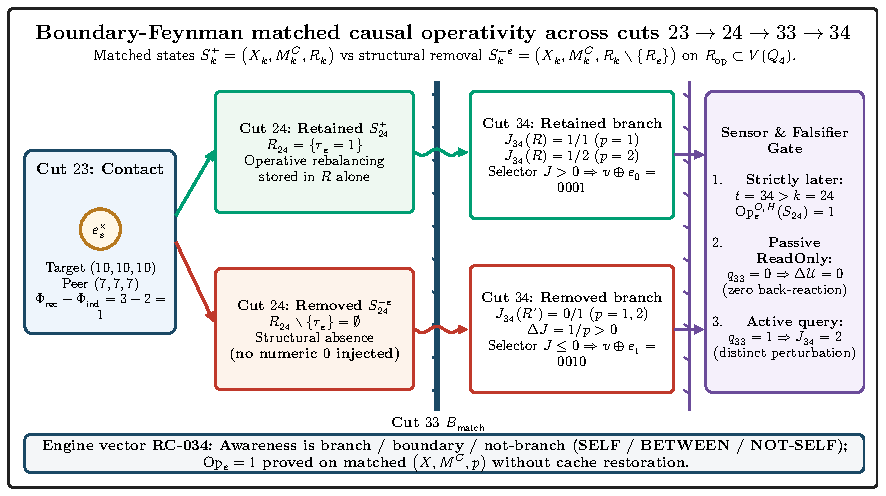
\includegraphics[width=0.92\linewidth,height=0.78\textheight,keepaspectratio]{figures/generated/awareness-matched-operativity-feynman.pdf}
\caption{Boundary-Feynman matched-state operativity walk $S_k^+=(X_k,M_k^C,R_k)$ versus structural removal $S_k^{-e}=(X_k,M_k^C,R_k\setminus\{R_e\})$, strictly-later cut-$34$ branching, and passive sensor zero-perturbation wall (\texttt{RC-034}, \texttt{awareness\_operativity\_dec\_walk.csv}).}
\label{fig:manual-awareness-matched-feynman}
\end{figure}

\begin{table}[H]
\centering
\caption{Engine-bound matched-state retained-relation operativity and passive-sensor D.E.C. ledger (\texttt{RC-034}, live from \texttt{awareness\_operativity\_dec\_walk.csv}).}
\label{tab:manual-awareness-dec-ledger}
{\scriptsize
\begin{tabular}{>{\raggedleft\arraybackslash}p{0.050\linewidth}>{\raggedright\arraybackslash}p{0.125\linewidth}>{\raggedright\arraybackslash}p{0.133\linewidth}>{\centering\arraybackslash}p{0.050\linewidth}>{\centering\arraybackslash}p{0.053\linewidth}>{\centering\arraybackslash}p{0.050\linewidth}>{\raggedleft\arraybackslash}p{0.074\linewidth}>{\centering\arraybackslash}p{0.050\linewidth}>{\raggedright\arraybackslash}p{0.240\linewidth}}
\toprule
Cut $k$ & Branch mode & State $S_k$ & $v$ & $e$ & $v_e$ & $J_k$ & $\operatorname{adm}$ & Route / operativity audit \\
\midrule
23 & \texttt{shared\_\allowbreak{}contact} & \texttt{(\allowbreak{}X\_\allowbreak{}23,\allowbreak{} M\_\allowbreak{}23\textasciicircum{}C,\allowbreak{} \{\})} & \texttt{0000} & \texttt{e\_\allowbreak{}cross} & \texttt{0000} & \texttt{0/\allowbreak{}1} & 1 & \texttt{recurrent\_\allowbreak{}3\_\allowbreak{}minus\_\allowbreak{}indep\_\allowbreak{}2} \\
24 & \texttt{S\_\allowbreak{}plus\_\allowbreak{}retained} & \texttt{(\allowbreak{}X\_\allowbreak{}24,\allowbreak{} M\_\allowbreak{}24\textasciicircum{}C,\allowbreak{} \{r\_\allowbreak{}e=1\})} & \texttt{0000} & \texttt{0\_\allowbreak{}H} & \texttt{0000} & \texttt{0/\allowbreak{}1} & 1 & \texttt{commit\_\allowbreak{}r\_\allowbreak{}e\_\allowbreak{}to\_\allowbreak{}R\_\allowbreak{}24} \\
24 & \texttt{S\_\allowbreak{}minus\_\allowbreak{}e\_\allowbreak{}removed} & \texttt{(\allowbreak{}X\_\allowbreak{}24,\allowbreak{} M\_\allowbreak{}24\textasciicircum{}C,\allowbreak{} \{\})} & \texttt{0000} & \texttt{0\_\allowbreak{}H} & \texttt{0000} & \texttt{0/\allowbreak{}1} & 1 & \texttt{structural\_\allowbreak{}absence\_\allowbreak{}no\_\allowbreak{}zero\_\allowbreak{}fill} \\
33 & \texttt{matched\_\allowbreak{}boundary\_\allowbreak{}p1} & \texttt{S\_\allowbreak{}33\textasciicircum{}+\allowbreak{} vs S\_\allowbreak{}33\textasciicircum{}\{-e\}} & \texttt{0000} & \texttt{0\_\allowbreak{}H} & \texttt{0000} & \texttt{1/\allowbreak{}1 vs 0/\allowbreak{}1} & 1 & \texttt{matched\_\allowbreak{}X\_\allowbreak{}M\_\allowbreak{}pressure\_\allowbreak{}p1} \\
34 & \texttt{response\_\allowbreak{}p1\_\allowbreak{}retained} & \texttt{S\_\allowbreak{}34\textasciicircum{}+\allowbreak{}(\allowbreak{}p=1)} & \texttt{0000} & \texttt{e0} & \texttt{0001} & \texttt{1/\allowbreak{}1} & 1 & \texttt{selector\_\allowbreak{}pos\_\allowbreak{}branch\_\allowbreak{}0001\_\allowbreak{}Op1} \\
34 & \texttt{response\_\allowbreak{}p1\_\allowbreak{}removed} & \texttt{S\_\allowbreak{}34\textasciicircum{}\{-e\}(\allowbreak{}p=1)} & \texttt{0000} & \texttt{e1} & \texttt{0010} & \texttt{0/\allowbreak{}1} & 1 & \texttt{selector\_\allowbreak{}nonpos\_\allowbreak{}branch\_\allowbreak{}0010\_\allowbreak{}Op1} \\
34 & \texttt{response\_\allowbreak{}p2\_\allowbreak{}and\_\allowbreak{}sensor} & \texttt{S\_\allowbreak{}34\textasciicircum{}+\allowbreak{}(\allowbreak{}p=2,\allowbreak{} q=0)} & \texttt{0000} & \texttt{e0} & \texttt{0001} & \texttt{1/\allowbreak{}2} & 1 & \texttt{passive\_\allowbreak{}sensor\_\allowbreak{}delta\_\allowbreak{}0\_\allowbreak{}1\_\allowbreak{}active\_\allowbreak{}q\_\allowbreak{}2\_\allowbreak{}1} \\
\bottomrule
\end{tabular}
}
\end{table}
